\documentclass[a4paper, 11pt]{article}
\usepackage[english, spanish, mexico]{babel}
\selectlanguage{spanish}
\usepackage[english]{isodate}


%
% Cargar el archivos de definiciones de la plantilla (debe estar en el mismo directorio
%
%%Paquetes
\usepackage[T1]{fontenc} % Codificación de fuente
\usepackage{lmodern} % Fuente compatible
\usepackage{graphicx}
\usepackage{float}
%\usepackage{xcolor}
\usepackage{ragged2e}
\usepackage{amssymb}
\usepackage{algorithm}
\usepackage{algpseudocode}
\usepackage{listings}
\usepackage[table]{xcolor}

\definecolor{codegreen}{rgb}{0,0.6,0}
\definecolor{codegray}{rgb}{0.5,0.5,0.5}
\definecolor{codepurple}{rgb}{0.58,0,0.82}
\definecolor{backcolour}{rgb}{0.95,0.95,0.92}

\lstdefinestyle{mystyle}{
    backgroundcolor=\color{backcolour},   
    commentstyle=\color{codegreen},
    keywordstyle=\color{magenta},
    numberstyle=\tiny\color{codegray},
    stringstyle=\color{codepurple},
    basicstyle=\ttfamily\footnotesize,
    breakatwhitespace=false,         
    breaklines=true,                 
    captionpos=b,                    
    keepspaces=true,                 
    numbers=left,                    
    numbersep=5pt,                  
    showspaces=false,                
    showstringspaces=false,
    showtabs=false,                  
    tabsize=2
}

\lstset{style=mystyle}

% requiere texlive-science
%\usepackage{algorithm2e}
%\usepackage[ruled,vlined,spanish]{algorithm2e}
%\usepackage{alghorithmic}
%\usepackage{verbatim}
\usepackage[utf8]{inputenc}
% colores en tablas
\usepackage{colortbl}
\usepackage{array}
\usepackage[table]{xcolor}
% ligas en el índice
\usepackage{color}
\usepackage{hyperref}
\hypersetup{
    colorlinks=true,
    linkcolor=naranjauam3,
    %urlcolor=blue, %el color mas usado para ligas
    urlcolor=naranjauam2,
    linktoc=all,
    %linkbordercolor = {white}, % es el color más usado
    citecolor=naranjauam
}
%
%%% Definiciones
%
% color naranja institucional UAM-C
\definecolor{naranjauam}{HTML}{F08200}
% variaciones del naranja institucional
\definecolor{naranjauam2}{HTML}{FF4000}
\definecolor{naranjauam3}{HTML}{B43104}
\gdef \LogoUAMC{%
{
\includegraphics[width=0.5\textwidth]{Plantilla/logoVar7Cua.png}\par}
}
\gdef \logosDTIDCCD{%
    {
\includegraphics[width=0.25\textwidth,height=1.2cm]{Plantilla/logoCCD.png}}
    \hspace{0.15\textwidth}
    {
\includegraphics[width=0.25\textwidth]{Plantilla/tsi_horizontal.png}}
    \hspace{0.15\textwidth}
    {
\includegraphics[width=0.1\textwidth]{Plantilla/logoDTI.png}\par}
    
}
\gdef \asesor{\small{Asesora: Nombre completo}}
\gdef \correo#1{\texttt{#1@cua.uam.mx}}
\gdef \LTSI{%
    {\scshape\small{LIC. EN TECNOLOGÍAS Y SISTEMAS DE INFORMACIÓN \par}}%
}
\gdef \DTI{%
    {\scshape DEPARTAMENTO DE TECNOLOGÍAS DE LA INFORMACIÓN \par}
}
\gdef \dti{%
    {\scshape Departamento de Tecnologías de la Información}
}
\gdef \dccd{%
    {\scshape División de Ciencias de la Comunicación y Diseño}
}
\gdef \autor#1#2{%
    \vfill
%{\Large Autor: \par}
    {\Large #1 \par}
    {\correo{#2}}
    \vfill
    {\asesor}
    \vfill
}
\gdef \tituloPTUno#1{%
    {\scshape\Huge #1 \par}
    \vspace{2cm}
    {\itshape\Large Proyecto Terminal \par}
 }%
 \gdef \tituloPTDos#1{%
    {\scshape\Huge #1 \par}
    \vspace{
    2.5cm}
    {\itshape\Large Informe PT2 \par}
 }%
 \gdef \tituloPTTres#1{%
    {\scshape\Huge #1 \par}
    \vspace{1.5cm}
    {\itshape\Large Proyecto Terminal \par}
 }%
 \gdef \carreraDepto{%
 \DTI
\vspace{1cm}
\LTSI
 }
 
\renewcommand{\spanishabstractname}{Resumen}
\renewcommand{\spanishcontentsname}{Índice}
% Fechas en español
\renewcommand{\today}{\ifnum\number\day<10 0\fi \number\day \space%
\ifcase \month \or Enero\or Febrero\or Marzo\or Abril\or Mayo%
\or Junio\or Julio\or Agosto\or Septiembre\or Octubre\or Noviembre\or Diciembre\fi, %
\number \year}

\newcommand{\hipotesis}[1]{%
%\textbf{Hipótesis} \par
\noindent
{\color{naranjauam} \rule{\linewidth}{0.5mm}}
%\fcolorbox{white}{yellow}{%
\begin{quotation}
{\textbf{#1}\par}%
\end{quotation}
%}
\noindent
{\color{naranjauam} \rule{\linewidth}{0.5mm}}
}
% Definiciones autonumeradas
\newtheorem{definicion}{Def.}
 
\renewcommand{\lstlistingname}{Código}% Listing -> Código

%%%%%% Inicio del documento
\begin{document}
% Apariencia de tablas
%\rowcolors{1}{green!90!yellow!80}{green!70!yellow!40}
\rowcolors{1}{naranjauam!90!yellow!80}{naranjauam!70!yellow!40}
%
% Portada
 \begin{titlepage}
\centering
% Logotipo de la UAM-C
\LogoUAMC
\vspace{1cm}
% Carrera y Depto
\carreraDepto
\vspace{2cm}
% Título del PT
\tituloPTUno{Título del proyecto}
% Apellidos, Nombre y Matrícula
\autor{Apellidos Nombre}{0123456789}
% Fecha actual
{\Large \printdate{2022-02-10} \par}
\vspace{1.5cm}
% Logotipos de unidad y depto
\logosDTIDCCD
\end{titlepage}

% Resumen en español
\begin{abstract}
Lorem ipsum dolor sit amet, consectetur adipiscing elit. Suspendiss blandit tellus at ipsum suscipit fringilla. Praesent placerat pretium lacus. Nunc blandit ultricies nisl, ut elementum augue pharetra at. Class aptent taciti sociosqu ad litora torquent per conubia nostra, per inceptos himenaeos. Sed maximus ante enim, a feugiat tellus hendrerit non. Pellentesque habitant morbi tristique senectus et netus et malesuada fames ac turpis egestas. Curabitur varius orci ut gravida volutpat. Ut mollis felis fermentum turpis sodales faucibus. Quisque nec magna et nisi vestibulum finibus nec in neque. Donec eu turpis non ex cursus iaculis.
\end{abstract}

%----- Si es necesario un resumen en otro idioma, si no lo es, puedes borrarlo.
\selectlanguage{english}
\begin{abstract}
Lorem ipsum dolor sit amet, consectetur adipiscing elit. Suspendisse blandit tellus at ipsum suscipit fringilla. Praesent placerat pretium lacus. Nunc blandit ultricies nisl, ut elementum augue pharetra at. Class aptent taciti sociosqu ad litora torquent per conubia nostra, per inceptos himenaeos. Sed maximus ante enim, a feugiat tellus hendrerit non. Pellentesque habitant morbi tristique senectus et netus et malesuada fames ac turpis egestas. Curabitur varius orci ut gravida volutpat. Ut mollis felis fermentum turpis sodales faucibus. Quisque nec magna et nisi vestibulum finibus nec in neque. Donec eu turpis non ex cursus iaculis.

\end{abstract}

\selectlanguage{spanish}
\newpage

% Índice
\tableofcontents
\newpage

%%% Contenido del documento
\section{Introducción}\label{Introd}
%----- Si no tienes subsecciones, utiliza este espacio para escribir tu introducción.
\subsection{Subtitulo}
%----- En esta subsección puedes escribir lo que quieras
Lorem ipsum dolor sit amet, consectetur adipiscing elit. Proin consequat et tortor hendrerit malesuada. Sed condimentum dictum arcu, vitae porta urna ultrices at. Nulla ac interdum lectus. Etiam vitae est in lorem suscipit vel ac nisi. Etiam iaculis porta nulla ut suscipit. Morbi efficitur pulvinar turpis, et convallis nulla lobortis a. Quisque ullamcorper quam sed eros congue, in consectetur enim vulputate. Duis pharetra sagittis odio et aliquet. Maecenas tincidunt ultricies accumsan. Aliquam sed lobortis tellus, at volutpat ex.

Proin eleifend lectus eget mi gravida fermentum. Sed bibendum pellentesque ipsum id blandit. Ut sit amet tempus ante. Proin a pulvinar enim. In ultrices nisi vitae odio pellentesque, id consequat neque dignissim. Suspendisse malesuada ex justo, gravida volutpat ante porta in. Morbi id dui velit. In non orci orci.

Interdum et malesuada fames ac ante ipsum primis in faucibus. Mauris condimentum volutpat metus nec sagittis. Aliquam vel ipsum sapien. Vestibulum ut felis id enim mattis aliquam. Nulla volutpat tincidunt risus, ac imperdiet ex dapibus a. Praesent mi nunc, sagittis quis dolor id, venenatis pharetra ex. Cras facilisis non enim sed consequat. Integer mollis sem nec sem ullamcorper, at facilisis eros tincidunt. Praesent tristique vitae felis placerat posuere. Nullam porttitor nunc sit amet mauris hendrerit pellentesque. Phasellus at varius massa, vitae tristique felis. Vestibulum id risus purus. Etiam aliquet dolor orci, at fringilla augue finibus et. Vestibulum nulla dui, elementum sed vulputate a, vestibulum quis mi.

%----- Marco Teórico
\section{Marco Teórico}\label{MarcoTeorico}

\subsection{Agregar imágenes}
Interdum et malesuada fames ac ante ipsum primis in faucibus. Mauris condimentum volutpat metus nec sagittis. Aliquam vel ipsum sapien. Vestibulum ut felis id enim mattis aliquam. Nulla volutpat tincidunt risus, ac imperdiet ex dapibus a. Praesent mi nunc, sagittis quis dolor id, venenatis pharetra ex. Cras facilisis non enim sed consequat. Integer mollis sem nec sem ullamcorper, at facilisis eros tincidunt. Praesent tristique vitae felis placerat posuere. Nullam porttitor nunc sit amet mauris hendrerit pellentesque. Phasellus at varius massa, vitae tristique felis. Vestibulum id risus purus. Etiam aliquet dolor orci, at fringilla augue finibus et. Vestibulum nulla dui, elementum sed vulputate a, vestibulum quis mi.


La arquitectura general de los sistemas de recomendación puede observarse en la Figura \ref{Figura01}.


\begin{figure}[H]
\centering
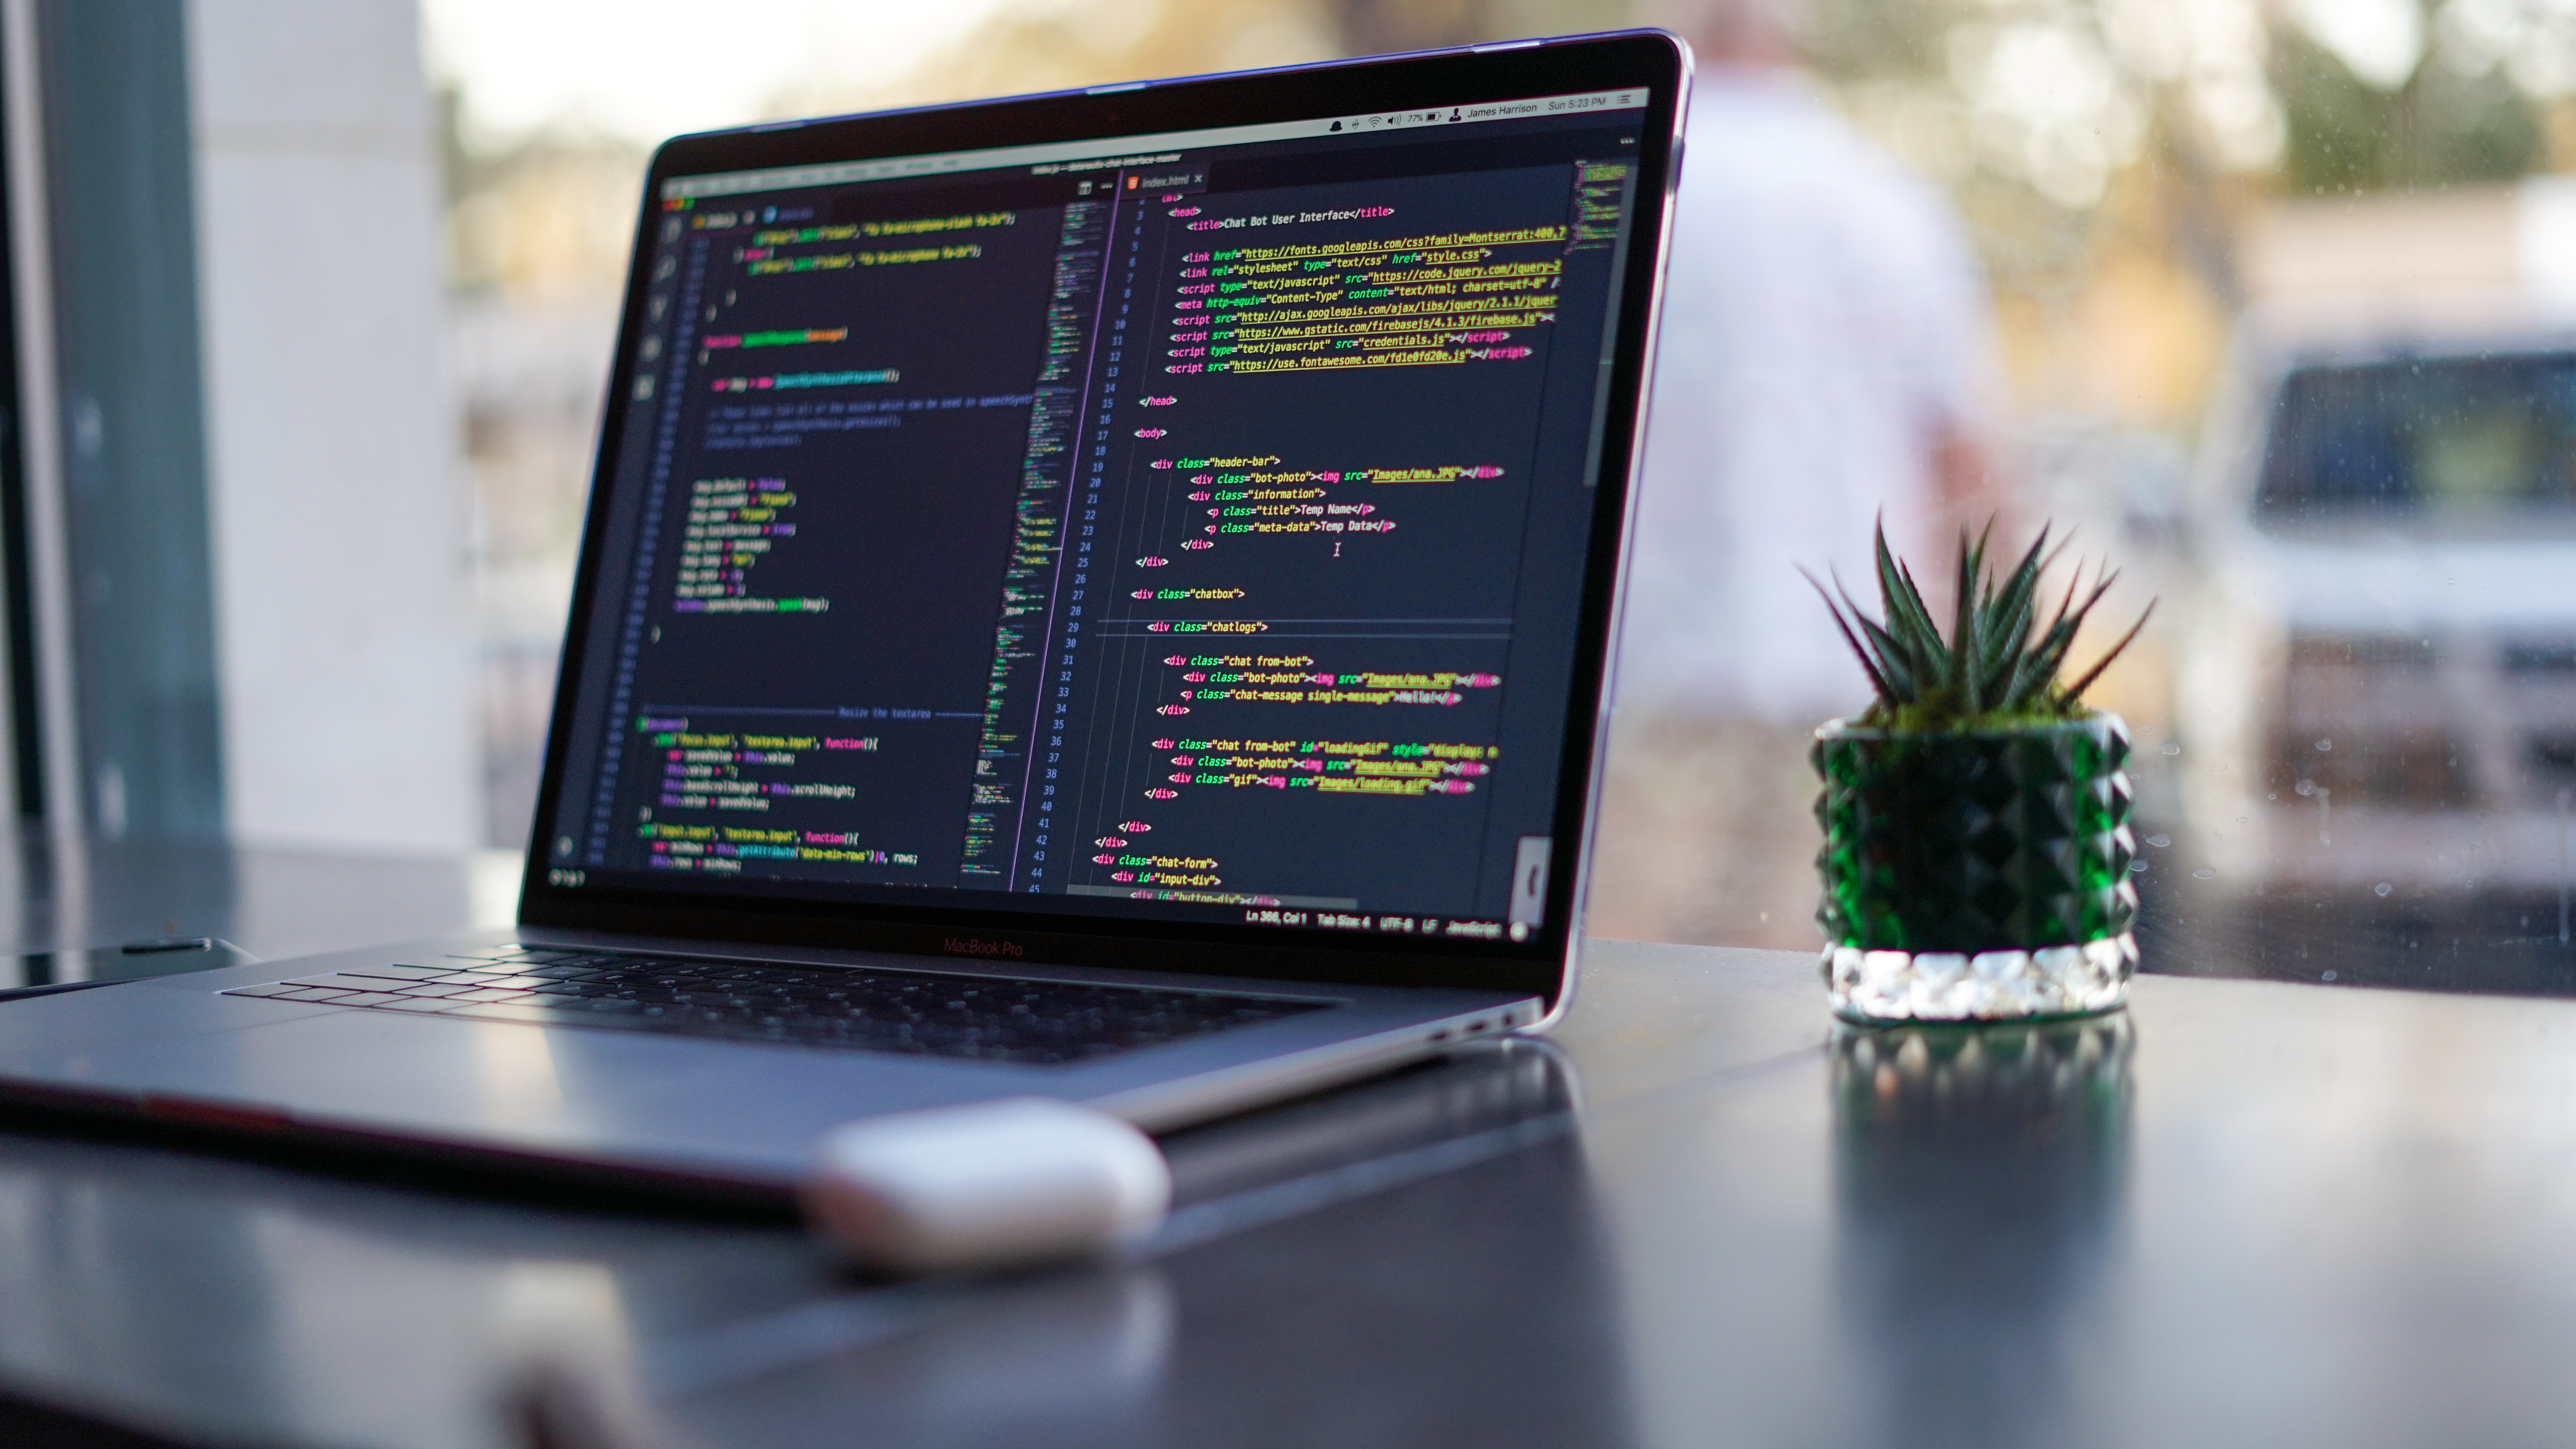
\includegraphics[width=12cm, height=7.3cm]{Doc/Figuras/Fig01.jpg}
\caption{Ejemplo de una imágen}
\label{Figura01}
\end{figure}
 
\subsubsection{Como citar}
Interdum et malesuada fames ac ante ipsum primis in faucibus. Mauris condimentum volutpat metus nec sagittis. Aliquam vel ipsum sapien.
Vestibulum ut felis id enim mattis aliquam. Nulla volutpat tincidunt risus, ac imperdiet ex dapibus a. Praesent mi nunc, sagittis quis dolor id, venenatis pharetra ex. 
Cras facilisis non enim sed consequat. Integer mollis sem nec sem ullamcorper, at facilisis eros tincidunt. Praesent tristique vitae felis placerat posuere. Nullam porttitor nunc sit amet mauris hendrerit pellentesque. 
Phasellus at varius massa, vitae tristique felis. Vestibulum id risus purus. Etiam aliquet dolor orci, at fringilla augue finibus et. Vestibulum nulla dui, elementum sed vulputate a, vestibulum quis mi \cite{niklas_python-agentspeak_2017}.

\subsection{Tablas}

\begin{table}[H]
\begin{center}
\begin{tabular}{| p{3cm} | p{7cm} |}
\hline
	Nombre & Descripción \\ \hline
	Elemento 01 & Vestibulum nulla dui, elementum sed vulputate a, vestibulum quis mi\\
	Elemento 02 & Vestibulum nulla dui, elementum sed vulputate a, vestibulum quis mi \\
	Elemento 03 & Vestibulum nulla dui, elementum sed vulputate a, vestibulum quis mi  \\ \hline
\end{tabular}
\caption{Ejemplo de una tabla}
\label{table:Tabla}
\end{center}
\end{table}

\subsection{Listas}
Si quieres colocar elementos en forma de lista como: 
\begin{itemize}
 \item{Ejemplos}
 \item{Distintos elementos}	
 \item{Puntos importantes}
\end{itemize}
Puedes leer el código de {\LaTeX} para que veas cómo hacerlas. \\

Existen tambien estas otras listas, las numeradas: 
\begin{enumerate}
	\item Primer elemento.
	\item Segundo.
	\item Ultimo.
\end{enumerate}


\section{Hipótesis}\label{Hipot}
%
\hipotesis{Vestibulum nulla dui, elementum sed vulputate a, vestibulum quis mi}

\section{Metodología}\label{Metod}
%
Lorem ipsum dolor sit amet, consectetur adipiscing elit. Suspendisse blandit tellus at ipsum suscipit fringilla. Praesent placerat pretium lacus. Nunc blandit ultricies nisl, ut elementum augue pharetra at. Class aptent taciti sociosqu ad litora torquent per conubia nostra, per inceptos himenaeos. Sed maximus ante enim, a feugiat tellus hendrerit non. Pellentesque habitant morbi tristique senectus et netus et malesuada fames ac turpis egestas. Curabitur varius orci ut gravida volutpat. Ut mollis felis fermentum turpis sodales faucibus. Quisque nec magna et nisi vestibulum finibus nec in neque. Donec eu turpis non ex cursus iaculis. 

\section{Código Fuente}
Si deseas agregar el código fuente o secciones de este al documento lo puedes hacer de la siguiente manera: 
\begin{lstlisting}[language=Python, caption=Código Python {\tt main.py},label={lst:main}]
import numpy as np

matrix1 = np.matrix('1 2 3; 4 5 6; 7 8 9')
print (matrix1)

\end{lstlisting} 

\subsection{Manual de usuario}
%----- Manual de usuario.
Lorem ipsum dolor sit amet, consectetur adipiscing elit. Suspendisse blandit tellus at ipsum suscipit fringilla. Praesent placerat pretium lacus. Nunc blandit ultricies nisl, ut elementum augue pharetra at. Class aptent taciti sociosqu ad litora torquent per conubia nostra, per inceptos himenaeos. Sed maximus ante enim, a feugiat tellus hendrerit non. Pellentesque habitant morbi tristique senectus et netus et malesuada fames ac turpis egestas. Curabitur varius orci ut gravida volutpat. Ut mollis felis fermentum turpis sodales faucibus. Quisque nec magna et nisi vestibulum finibus nec in neque. Donec eu turpis non ex cursus iaculis.

\section{Conclusión y trabajo futuro}
%----- Conclusión
Lorem ipsum dolor sit amet, consectetur adipiscing elit. Suspendisse blandit tellus at ipsum suscipit fringilla. Praesent placerat pretium lacus. Nunc blandit ultricies nisl, ut elementum augue pharetra at. Class aptent taciti sociosqu ad litora torquent per conubia nostra, per inceptos himenaeos. Sed maximus ante enim, a feugiat tellus hendrerit non. Pellentesque habitant morbi tristique senectus et netus et malesuada fames ac turpis egestas. Curabitur varius orci ut gravida volutpat. Ut mollis felis fermentum turpis sodales faucibus. Quisque nec magna et nisi vestibulum finibus nec in neque. Donec eu turpis non ex cursus iaculis.

\section{Disponibilidad del código} 
%------ Repositorio del proyecto
Para más información del proyecto: 
\begin{itemize}
	\item Sitio web: \href{http://lab-ltsi.cua.uam.mx}{http://lab-ltsi.cua.uam.mx}
	\item Correo electrónico: \href{mailto:someone@cua.uam.mx}{0123456789@cua.uam.mx}
\end{itemize}\ \

\section{Publicaciones}
%----- Lista de publicaciones
\begin{itemize}
	\item Información sobre la publicación, \emph{Conferencia}, 2023.
\end{itemize}


% Bibliografía
%----- Referencias con el formato de la IEEE
\bibliographystyle{ieeetr}
% Definir, si se prefiere en archivo separado .bib
\bibliography{Referencias.bib}
% o definiendo cada referencia aquí mismo:
%\begin{thebibliography}{}
%\bibitem{} 
%\end{thebibliography}
%

\end{document}
